
\chapter{Metody vizualizace a porovnání}

Cílem této knihovny není pouze vizualizovat sekundární strukturu RNA, ale také
usnadnit analýzu rozdílů a podobností mezi více strukturami RNA. Proto jsme se
zaměřili na práci s radial diagramy, které nejlépe zobrazujou motivy struktury
a zároveň jsou nejpřirozenější reprezentací.

Kromě toho jsme viděli potenciál generování rozložení na základě vzorové
struktury, jak to dělá nástroj Traveler. Výstupem Traveleru je soubor ve
formátu JSON, který obsahuje informace o vzoru každého nukleotidu a provedených
úpravách - přidání, odebrání, přejmenování a přesunutí nukleotidu.

Například pokud bychom použili nástroj Varna na zobrazení následujících dvou
struktur musíme všechny podobnosti vypozorovat sami. 

\begin{figure}[H]
  \centering
  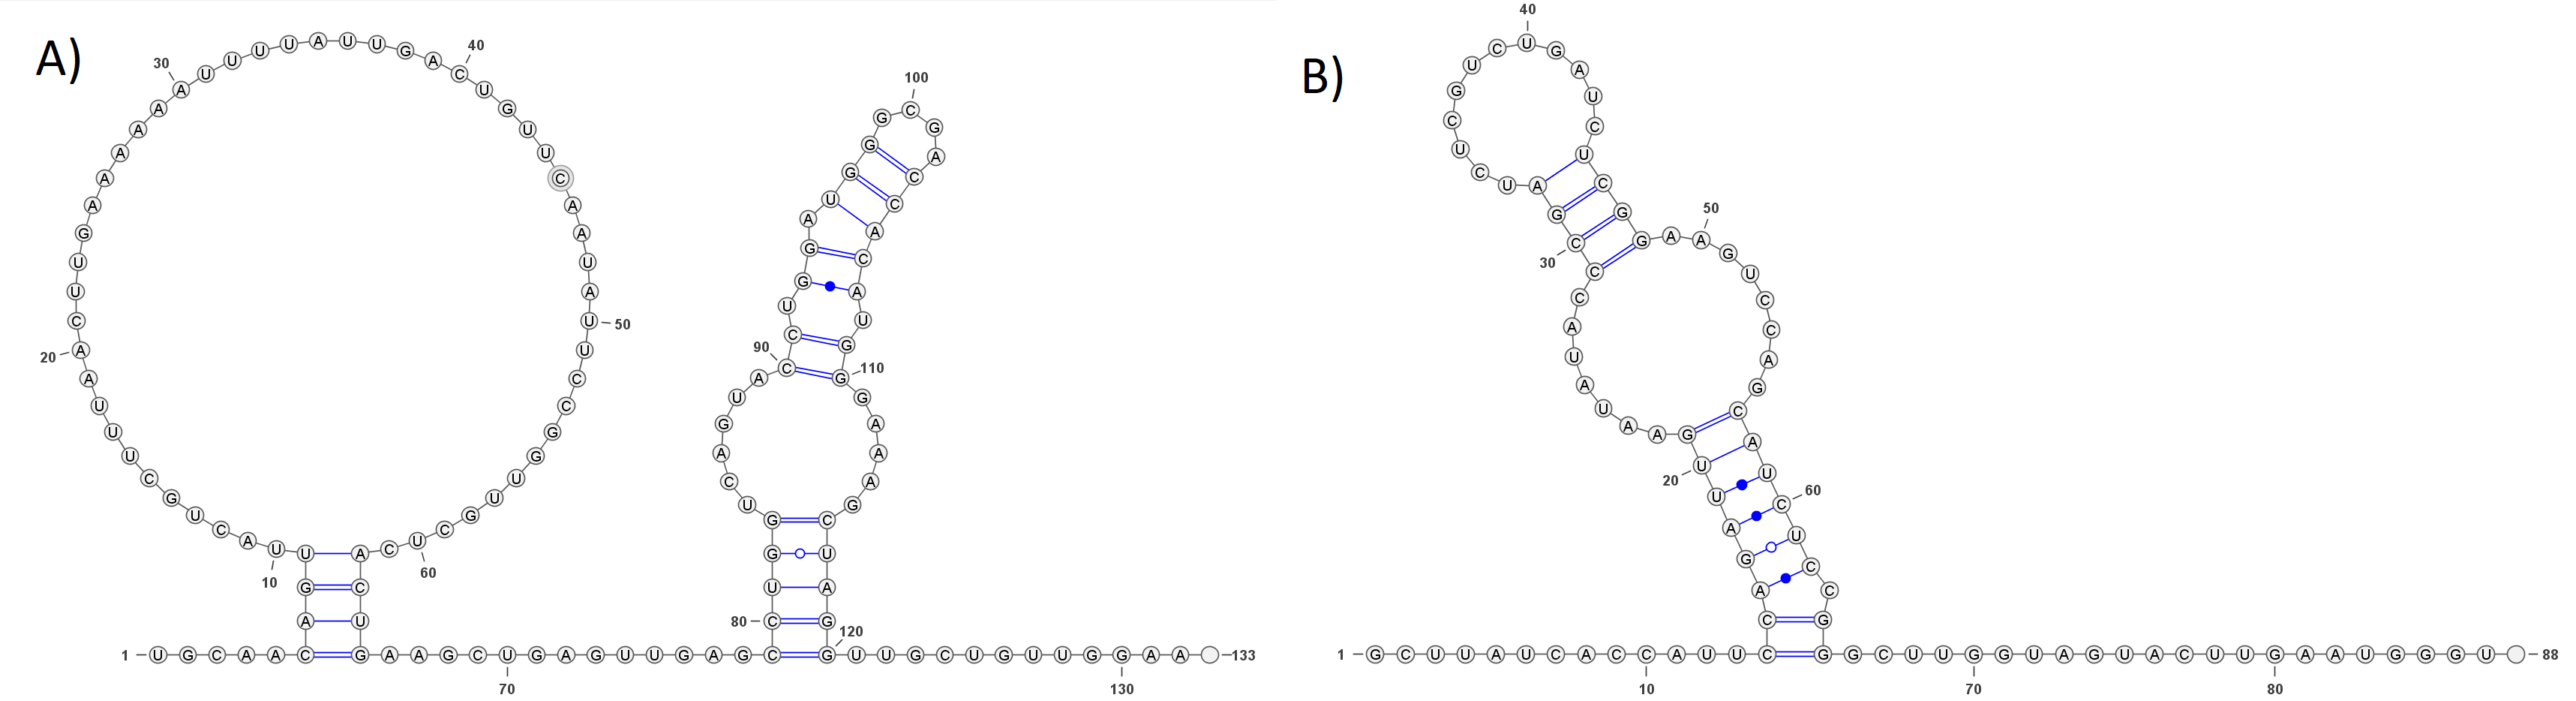
\includegraphics[width=140mm]{../img/kap02/intro/varna.png}
  \caption{Dvě sekundární RNA struktury s RNAcentral ID A) URS00006E712C, B)
  URS0000AB09C9.}
\end{figure}

Sice není těžké vypozorovat některé podobné motivy, ale není na první pohled
jasná podobnost sekvence.

Na generování obou struktur používá nástroj Traveler stejnou vzorovou
strukturu, která je v tomto konkrétním případě podobná obou odvozeným
strukturám. Podobnost odvozených struktur ke vzorové je až na vyjímky běžná, a
proto jsme se rozhodli tuto podobnost předpokládat. Následující obrázek je
vizualizace stejných struktur, za použití nástroje Traveler spolu se vzorovou
strukturou.

\begin{figure}[H]
  \centering
  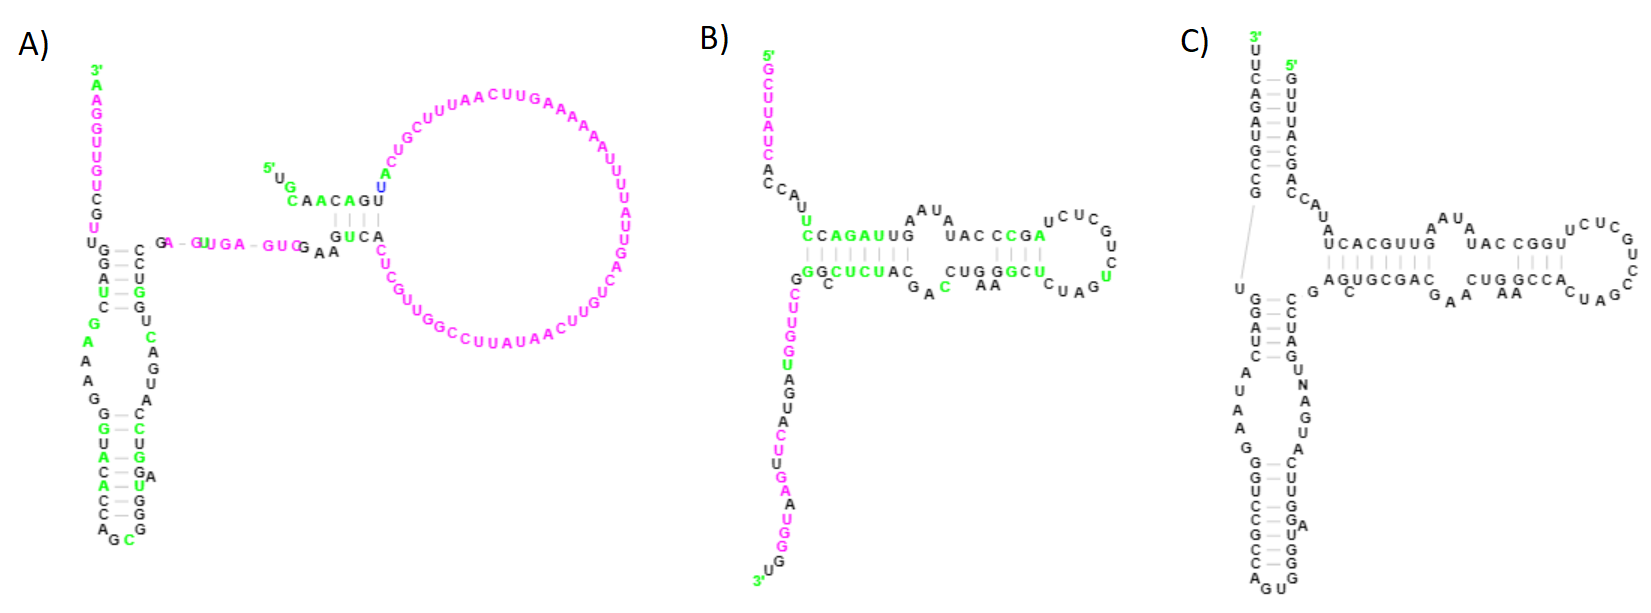
\includegraphics[width=140mm]{../img/kap02/intro/alignMotivationTemplate.png}
  \caption{Dvě sekundární RNA struktury s RNAcentral ID A) URS00006E712C, B)
  URS0000AB09C9 vygenerované nástrojem Traveler a C) vzorové sekundární RNA
  struktury d.5.e.S.oshimae.}
\end{figure}

Přidáním struktury, ze které jsou obě sturktury odvozené, je mnohem jasnější,
na která místa koukat pří hledání podobností a rozdílů. Přesto nemusí být
nějaká podobnost hned jasná, a proto jsme se zaměřili na způsoby, jak znázornít
mapování nukleotidů na vzorovou strukturu.

\section{Důsledek využívaní vzorové struktury}

Využívání vzorové struktury pro analýzu má zřejmý a důležitý důsledek. Náš
nástroj usnadňuje analýzu $N$ struktur, které byly vygenerované ze stejné
vzorové struktury. 

Protože Traveler umožňuje zadat, která vzorová struktura se má použít pro
generování je teoreticky možné, porovnávat jakékoliv dvě sekundární RNA
struktury, pokud bude jejich rozložení vygenerované na základě stejné vzorové
struktury. Pokud se ale pokusíme vygenerovat rozložení struktury pomocí vzorové
struktury, která je úplně jiná, nebude existovat žádná podobnost se vzorovou
strukturou, a tím pádem naše metody, které spoléhají na podobnost vzorové
struktury s vygenerovanou nebudou užitečné.

\section{Překládání struktur}

Vygenerované sekundární struktury jsou podobné vzorové struktuře, a tím pádem
bývají podobné i ostatním vygenerovaným strukturám ze stejné vzorové struktury.
Dává proto smysl se pokusit struktury přes sebe přeložit, aby se spojily
společné části a vynikly rozdíly. Pouhým přeložením podobných struktur přes
sebe však získáme výsledek, který neposkytuje příliš zajímavé informace a je
málo přehledný.

\begin{figure}[H]
  \centering
  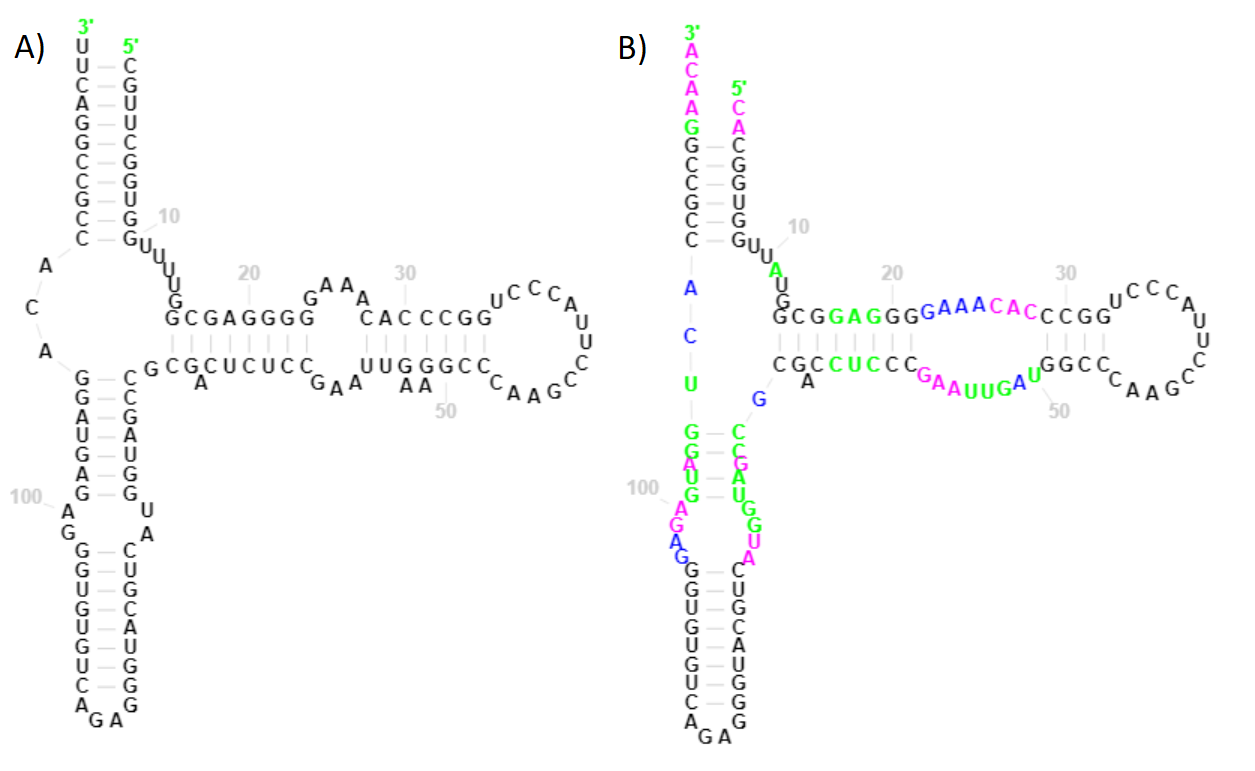
\includegraphics[width=140mm]{../img/kap02/align/structures.png}
  \caption{A) Struktura s RNAcentral ID URS00000B9D9D vygenerovaná nástrojem
  Traveler pomocí B) vzorové struktury d.5.b.A.madurae vedle sebe.}
\end{figure}

\begin{figure}[H]
  \centering
  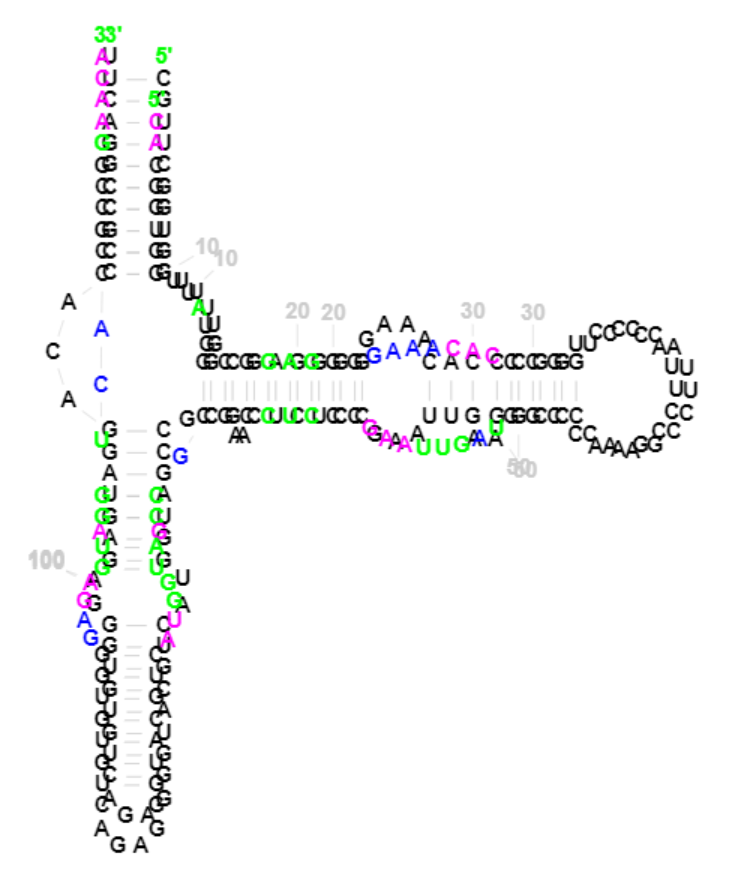
\includegraphics[height=90mm]{../img/kap02/align/unaligned.png}
  \caption{A) Struktura s RNAcentral ID URS00000B9D9D vygenerovaná nástrojem
  Traveler pomocí B) vzorové struktury d.5.b.A.madurae přeložené přes sebe.}
\end{figure}

\subsection{Zarovnání}

Je potřeba najít způsob, jak řešit problém přesunu a zarovnání struktury,
protože manuální manipulace pomocí přetažení myší nebo zadávání pozice může být
zbytečně obtížná, zejména pokud se snažíme dosáhnout přesného zarovnání. Proto
je velmi užitečné umožnit zarovnání sekundární RNA struktury na konkrétní
nukleotid nebo skupinu nukleotidů ze vzorové struktury. 

Pokud je vybrán vzorový nukleotid $v$ pro nukleotid $n$ z ostatních struktur,
jehož vzor je $v$, je celá struktura přesunuta tak, aby se nukleotidy $v$ a $n$
překrývaly. 

\subsubsection{Skupiny nukleotidů}

Pokud se snažíme najít větší skupinu nukleotidů, na které chceme strukturu
zarovnat, koukáme se na posunutí pro konkrétní nukleotidy a následně vybereme
buď posunutí které zarovná nejvíc nukleotidů nebo to které zarovná skupinu
nukleotidů které jsou v části struktury, která nás právě zajímá.

Pro hledání konkrétního posunutí pro zarovnání jsme použili naivní způsob,
který nezaručuje nejlepší možné zarovnání, ale zároveň je poměrně přímočarý a
dává rozumné výsledky, díky již zmíněné podobnosti struktur.

Postupně se prochází každá struktura. V první iteraci se porovná pozice každého
nukleotidu s pozicí ve vzorové struktuře. Na základě pozice se roztřídí
nukleotidy. Třídění funguje tak, že do stejné skupiny indexované posunutím se
přidají všechny vzorové nukleotidy, na které se struktura zarovná daným posunutím.
Na konci první iterace se skupiny, které jsou menší než $x$ odeberou.

V druhé iteraci se postupuje podobně, ale používají se poslední vytvořené
skupiny na filtrování, tím se snažíme docílit, zarovnání na stejné nukleotidy.
Filtrování pomocí skupin ingoruje všechny nukleotidy, jejiž vzor není v nějaké
skupině, pomocí které filtrujeme. Pokud během iterace nevzniknou žádné skupiny,
řeší se iterace daná iterace zvlášť bez filtrování.

\begin{figure}[H]
  \centering
  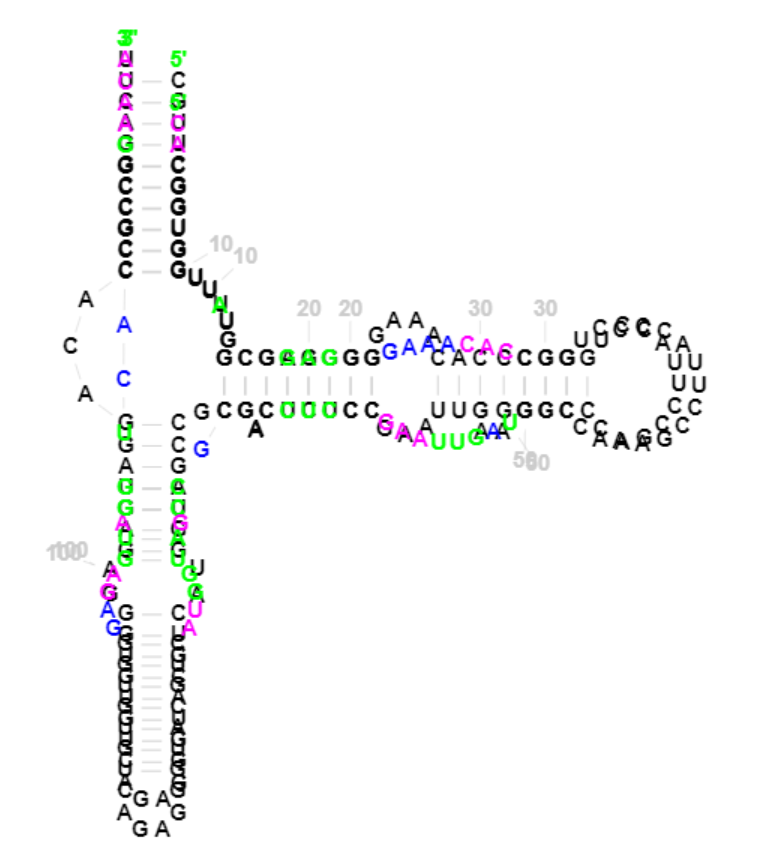
\includegraphics[height=90mm]{../img/kap02/align/alignedAlpha1.png}
  \caption{A) Struktura s RNAcentral ID URS00000B9D9D vygenerovaná nástrojem
  Traveler pomocí B) vzorové struktury d.5.b.A.madurae přeložené přes sebe a
  zarovnané.}
\end{figure}

\subsection{Průhlednost struktur}

V přeložených a zarovnaných strukturách nelze snadno rozeznat, které nukleotidy
jsou společné a překrývají se a které nejsou. Přidáním průhlednosti je možné
tuto situaci rozlišit, protože překrývající se nukleotidy budou mít sytější
barvu než ty, které se nepřekrývají.

\begin{figure}[H]
  \centering
  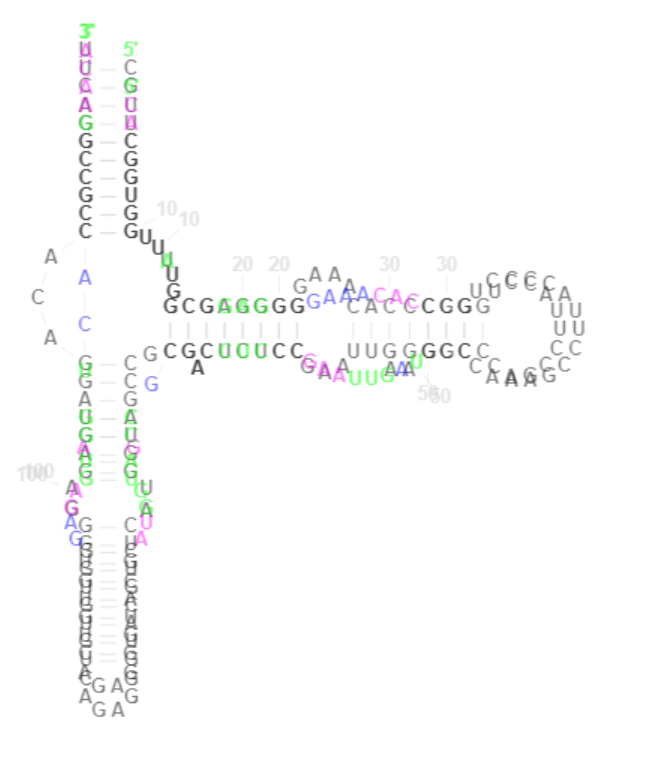
\includegraphics[height=90mm]{../img/kap02/align/aligned.png}
  \caption{A) Struktura s RNAcentral ID URS00000B9D9D vygenerovaná nástrojem
  Traveler pomocí B) vzorové struktury d.5.b.A.madurae přeložené přes sebe,
  zarovnané a s průhledností.}
\end{figure}

\subsection{Rozmazání struktur}

Zarovnávání struktur bohužel neřeší všechny výzvy. Výsledné obrázky se mohou
zdát rozmazané. To je způsobeno tím, že ačkoli má nukleotid vzorový nukleotid,
který je stejný, jeho pozice se může v rozložení mírně lišit v důsledku metody
generování dat. Tento fakt může způsobit, že popisky nukleotidů vypadají
rozmazaně.

Jako přímočaré řešení se může zdát posunoutí jednotlivých nukleotidů, které jsou
blízko sebe, aby dokonale překrývaly jejich vzory. Věříme, že by to vyřešilo
zmíněný problém bez významné deformace struktury.

\section{Obarvení struktur}

Vstupní data obsahují barevné označení nukleotidů. Slouží k lepšímu
zorientování se ve struktuře vzhledem ke vzorové struktuře. Jejich význam je
následující.

Černá barva značí, že nukleotid leží na poloze vzorového nukleotidu se stejným
názvem. Zelenou barvou jsou označený ty nukleotidy jejiž vzorový nukleotid bylo
třeba přejmenovat. Modrou barvou jsou vyznačený posunutý nukleotid. A poslední
růžovou barvu mají nově přidané nukleotidy.

\begin{figure}[H]
  \centering
  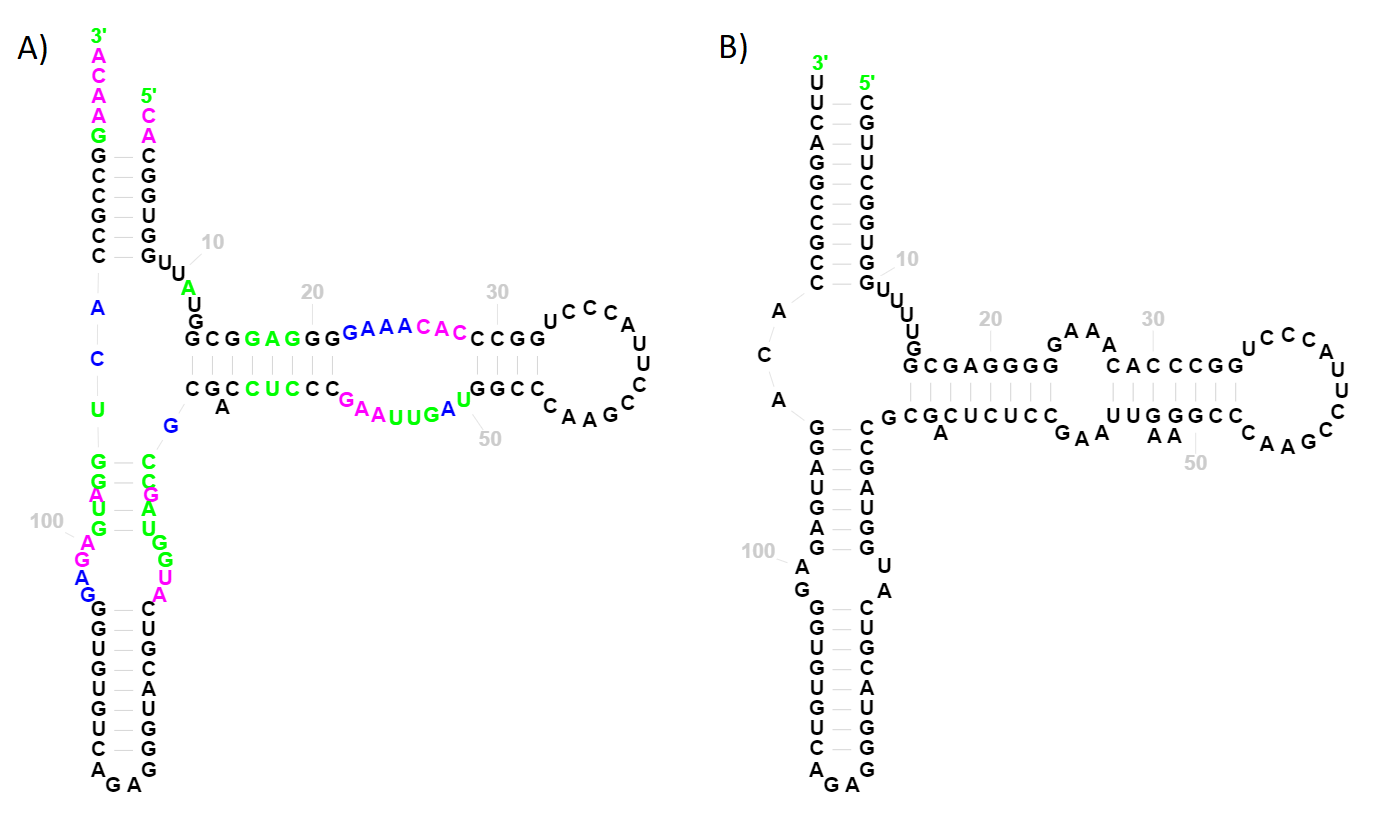
\includegraphics[width=140mm]{../img/kap03/inputDataColors.png}
  \caption{A) Struktura s RNAcentral ID URS00000B9D9D vygenerovaná nástrojem
  Traveler pomocí B) vzorové struktury d.5.b.A.madurae.}
\end{figure}

\section{Transformace na vzor}

Užitečnou metodou je transformace mezi vzorovou a cílovou strukturou. Každý
nukleotid, který má svůj vzorový nukleotid, se přemístí na pozici vzorového
nukleotidu a nukleotidy, které ve vzoru nejsou, jsou skryté. Tato metoda je
velmi užitečná pro práci s dvěma strukturami, které jsou si podobné, nebo pro
získání počátečního přehledu o tom, co je na co namapováno. 

Slabou stránkou této metody je její použití při práci s více než dvěma
strukturami nebo strukturami, které jsou velmi odlišné. V takových situacích se
na obrazovce děje mnoho věcí a je obtížné se soustředit a vypozorovat něco
užitečného.

\begin{figure}[H]
  \centering
  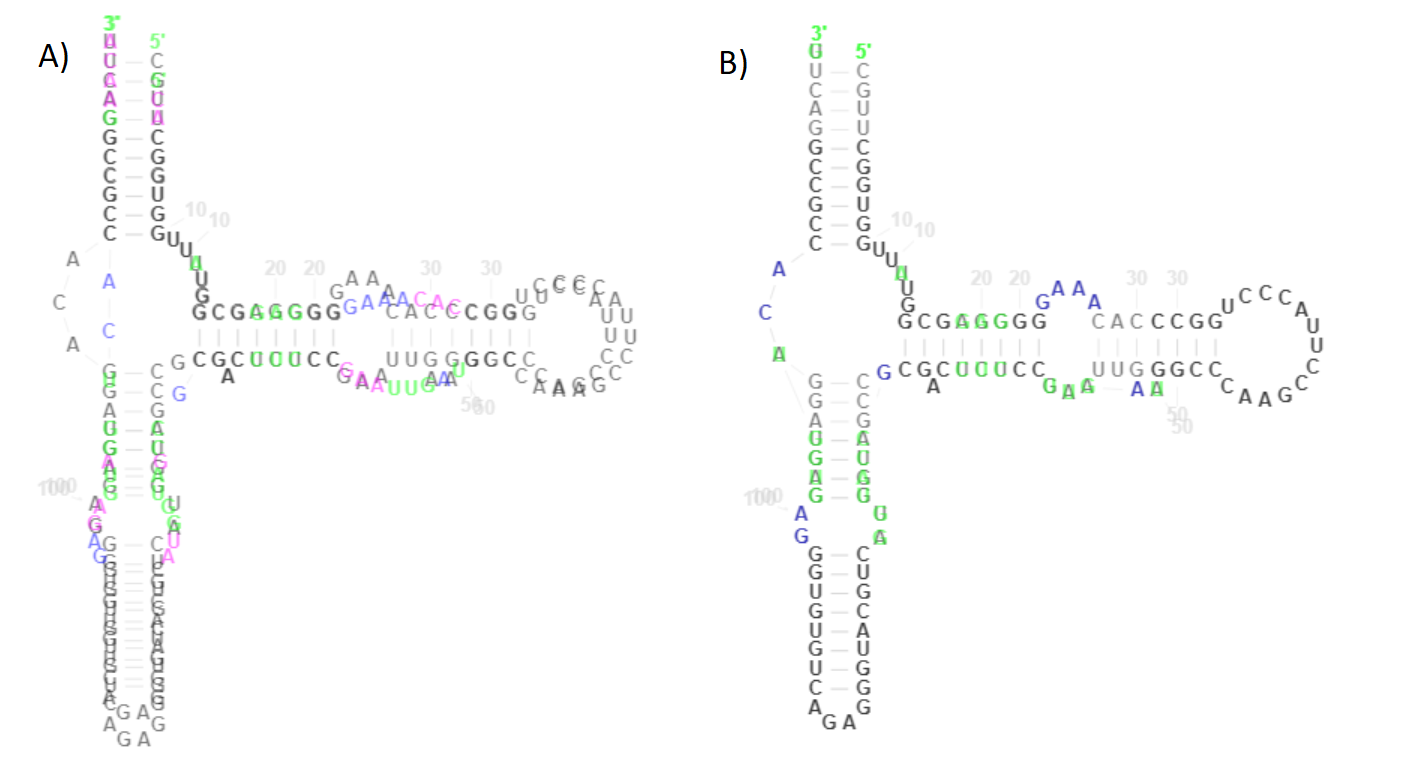
\includegraphics[width=140mm]{../img/kap02/animation.png}
  \caption{Struktura s RNAcentral ID URS00000B9D9D vygenerovaná nástrojem
  Traveler pomocí vzorové struktury d.5.b.A.madurae přeložené přes sebe A) před
  transformací a B) po transformaci.}
\end{figure}

\section{Mapovací čáry}

Vědomost o tom, který nukleotid se na co mapuje, může být důležitá pro odhalení
rozdílů a podobností mezi strukturami. V našem úsilí zprostředkovat tuto
informaci již před transformací na vzorovou sturkturu jsme přišli s čárami,
které spojují každý nukleotid s jeho vzorovým nukleotidem.

\begin{figure}[H]
  \centering
  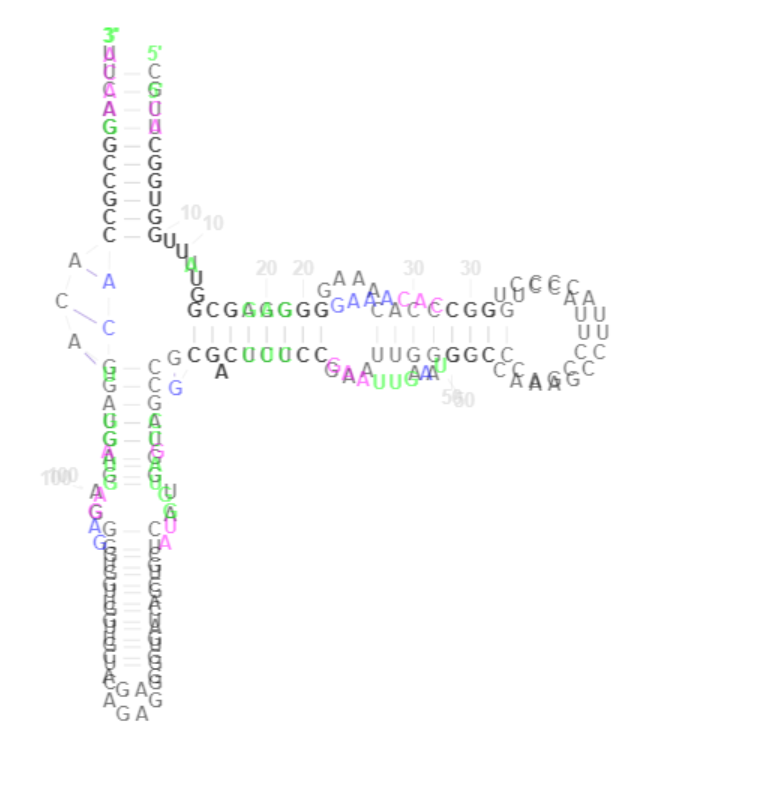
\includegraphics[height=90mm]{../img/kap02/mappingLines/small.png}
  \caption{Struktura s RNAcentral ID URS00000B9D9D vygenerovaná nástrojem
  Traveler pomocí vzorové struktury d.5.b.A.madurae přeložené přes sebe s
  mapovacíma čárama.}
\end{figure}

Bohužel tento způsob se zvětšující se velikostí struktury stáva velmi
nepřehledným, přesto si myslíme že můžou být užitečné.

\begin{figure}[H]
  \centering
  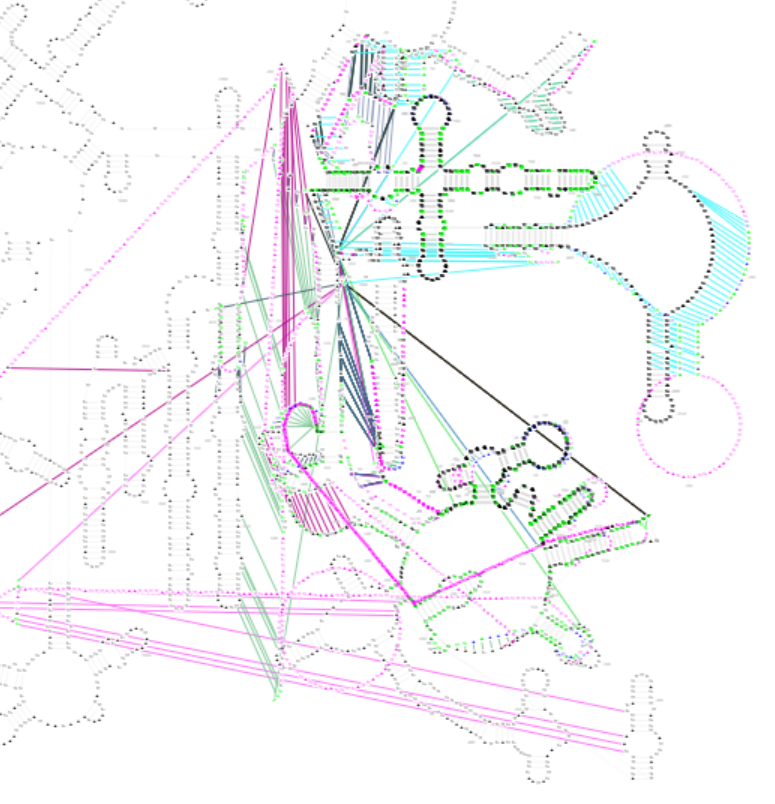
\includegraphics[height=100mm]{../img/kap02/mappingLines/big.png}
  \caption{Výřez z mnoha struktur vygenerovaných nástrojem Traveler pomocí vzorové struktury DD\_28S\_3D přeložených přes sebe s mapovacími čárami.
  Každá struktura má vlastní barvu mapovacích čar.}
\end{figure}

\section{Využití stromu}

V projektu Traveler byla použita stromová reprezentace pro sekundární RNA
strukturu, ve které je vnitřní vrchol, tedy má více jak jednu hranu, bázový pár
a listem, tedy má jednu nebo žádnou hranu, je nezpárovaný nukleotid. Strom pak
lze vytvořít následovně. První nepárové nukleotidy ze začátku a z konce přidáme
jako samostatné vrcholy. Potom jdeme postupně po bázových párech. První bázový
pár tvoří kořen. Další bázové páry připojujeme a tvoříme strom. Pokud narazíme
na nezpárovaný nukleotid přidáme ho jako list k poslednímu přidanému bázovému
páru. Větvení strukutry vyustí ve větvení stromu. 

\begin{figure}[H]
  \centering
  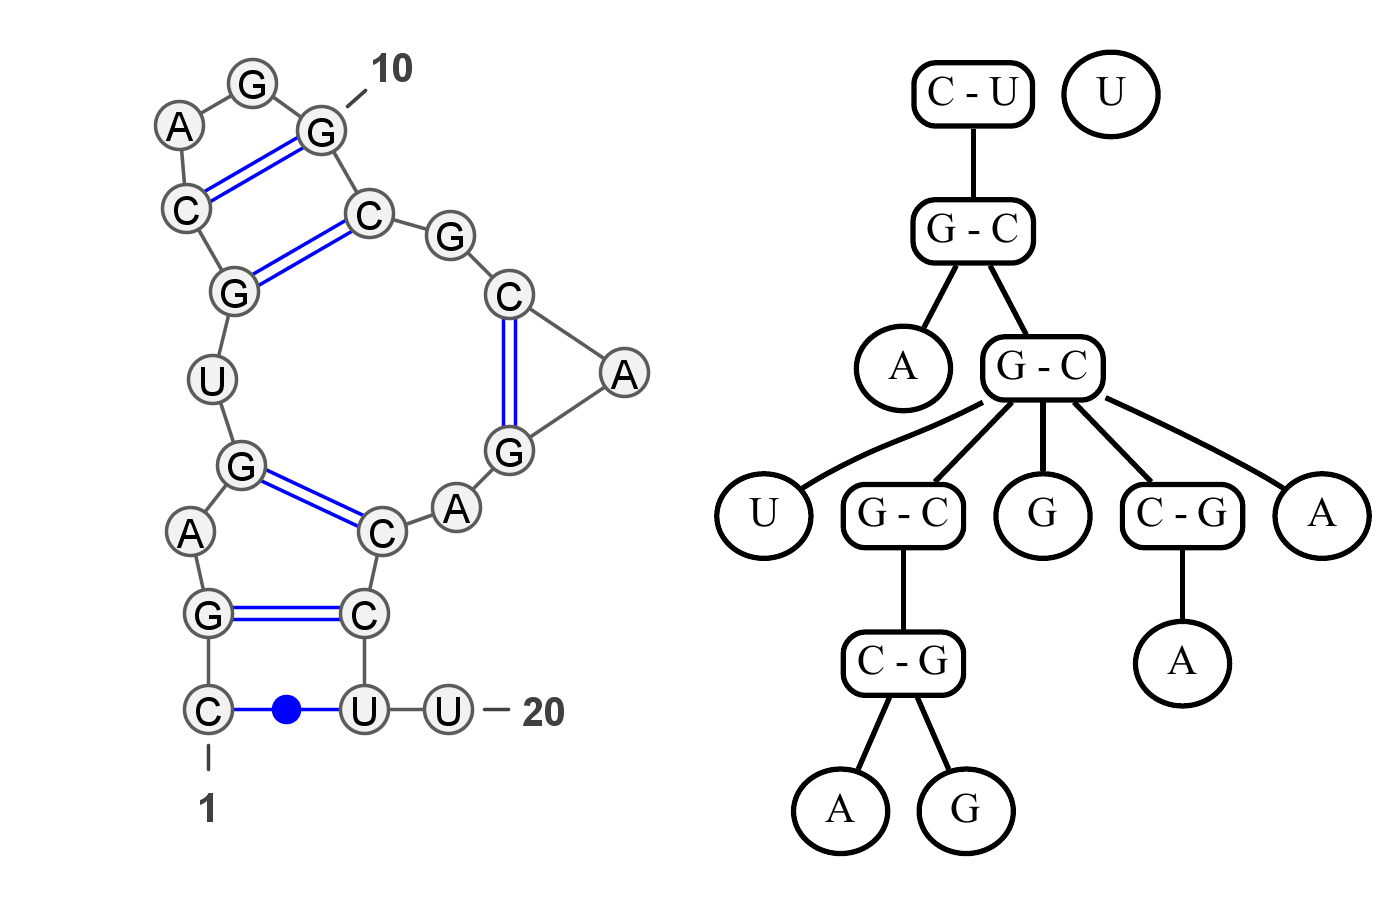
\includegraphics[width=140mm]{../img/kap02/tree/tree.png}
  \caption{Vlevo je uměle vytvořená struktura zobrazená nástrojem Varna. Vpravo je jeho stromová reprezentace.}
\end{figure}

Stromovu strukturu jsme neměli v úmyslu použít na nic konkrétního, ale chtěli
jsme prozkoumat možnosti lokálních transformací struktury pro dosažení
zarovnání více podobných částí, které jsou třeba jenom posunuté, jako je to
například v následující části dvou struktur, které jsou zarovnané dvouma
způsoby.

\begin{figure}[H]
  \centering
  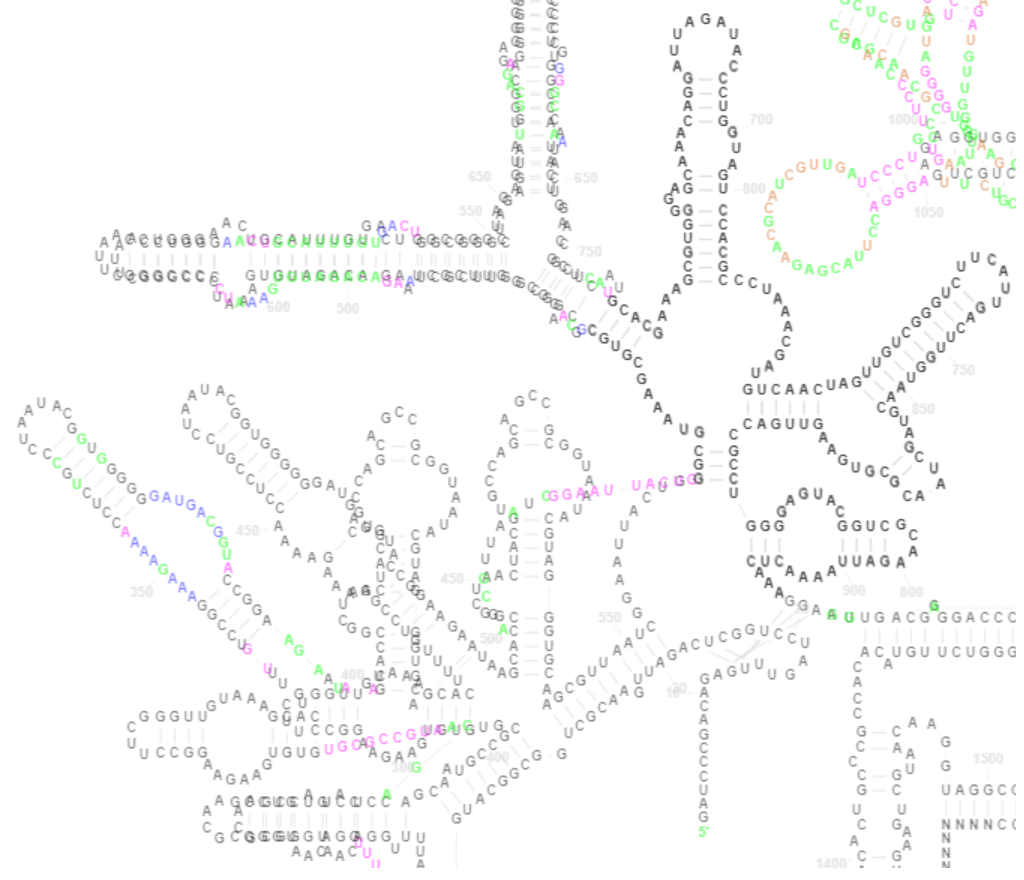
\includegraphics[height=100mm]{../img/kap02/tree/align1.png}
  \caption{První způsob zarovnání.}
\end{figure}

\begin{figure}[H]
  \centering
  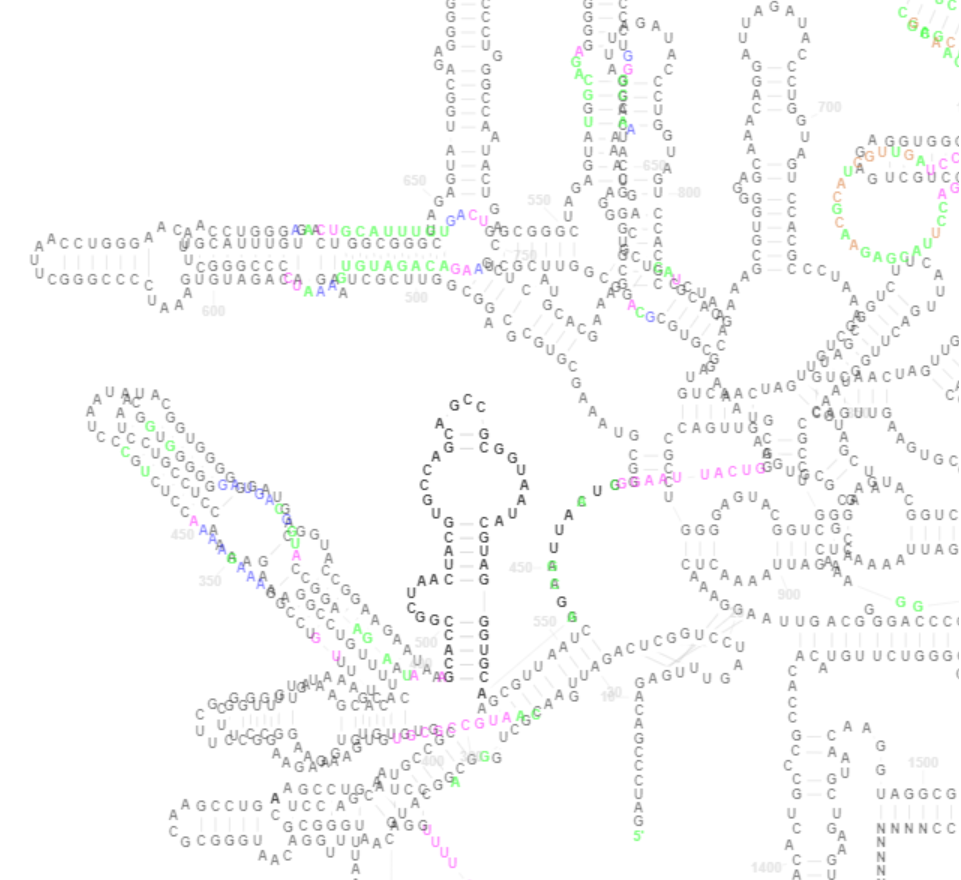
\includegraphics[height=100mm]{../img/kap02/tree/align2.png}
  \caption{Druhý způsob zarovnání.}
\end{figure}

Po zvážení jsme dospěli k názoru, že není možné provést úpravu struktury, která
by významně nedeformovala strukturu. Jakákoli úprava části struktury znamená
posunutí nějakého zbytku struktury, což může zasáhnout do jiné části. Proto by
bylo nezbytné odebrat některé nukleotidy. Ty, které nejvíce překážejí, jsou ty
přidané. Pokud bychom odebrali tyto přidané nukleotidy, dostali bychom se na
stejný výsledek jako s transformací struktury na vzorovou strukturu.

\section{Zvolené metody}

Naše knihovna přímo podporuje překládání a zarovnání struktur na konkrétní
nukleotid nebo skupinu nukleotidů bez zarovnání na úrovni jednotlivých
nukletidů pro odstranění rozmazání struktur. Lze transformovat struktury na
vzorovou strukturu a upravovat průhlednost struktur.
